%*******10********20********30********40********50********60********70********80

% For all chapters, use the newdefined chap{} instead of chapter{}
% This will make the text at the top-left of the page be the same as the chapter

\chap{Materials and Methods}\label{chap:materialsandmethods}
As anticipated in Section \ref{sec:roleofpediatrician} on page \pageref{sec:roleofpediatrician},  internationally adopted children in Italy get tested in one of 20 centers, one per region. In Friuli-Venezia Giulia, this center is placed in \textit{San Vito al Tagliamento}, where the data for this paper was collected. International adoptees are brought to this hospital by the adoptive parents as an autonomous decision or because they have been previously advised by adoption organizations or their trusted pediatrician. The child is hospitalized for just one day. This is the minimum time required in order to obtain all the necessary samples for laboratory examination (blood, stool, \textit{etc}\dots) and to complete all clinical evaluations while minimizing the stress the child must bear.

All 20 Italian adoption-focused centers follow the \textit{ad hoc} GLNBI diagnostic and aiding protocol,  in order to identify infectious diseases, nutritional deficiencies, immunization status, intestinal parasitosis, or other pathologies. These can be found in \cite{GNLBI1}, \cite{GNLBI2}, and \cite{GNLBI3}.

From \nth{1} January 2002 to \nth{31} December 2017 data was collected of all children evaluated by the \textit{San Vito al Tagliamento} GLNBI Center. Data regarding date of birth, sex, birthplace, arrival date in Italy, date of the first visit at our clinic and any possible health certificate they might have carried along were recorded for each child (family history, past and recent medical history, any previously performed laboratory test, vaccine certifications, \textit{etc}\dots) (see \cite{redbook}).\\
Laboratory blood tests included serological research of vaccine immunization (Diphtheria, Tetanus, Pertussis, Poliomyelitis, Rubella, Mumps and Measles), serological tests for ongoing or previous infections with HIV, Syphilis, HBV, HCV, blood count, erythrocyte sedimentation rate, serum protein electrophoresis, and dosing of blood sugar levels, creatinine, transaminase, ferritin, calcium, magnesium, phosphorus, alkaline phosphatase, vitamin D, and parathormone. Moreover, Mantoux test (PPD), aiming to evaluate any ongoing or previous tubercular infection, microbiological test on fecal samples for parasitological investigation, clinical urine tests, and thyroid hormone levels were performed.\\
Along with these laboratory tests, a complete physical examination for assessing the overall child health status was performed and, when facing potential specific pathology, a specialist’s visit (pediatric orthopaedist, dermatologist, otorhinolaryngologist, endocrinologist, surgeon, ECG or echocardiogram) were prescribed.

The aim of this study was to elaborate on the multitude of data this screening protocol provides, to understand and evaluate whether there might be space for simplification, revision, or stratification in the considered procedures. Over 17 years data was collected from every single child, in order to further uncover which disease affect these children and what can we do to treat them and to prevent short and long-term complications. Moreover, our research group, under the motto ``textit{Simplification through knowledge}", aimed at looking for every test and procedure that could be questioned and maybe halted, so to polish and refine the protocol at its finest. This was made through two main strategies: a profound re-evaluation of the meaning and reason of every test (see Section \ref{sec:worthwile?}), and the research for statistical correlations amongst parameters (discussed in Section \ref{sec:seekingforsupport}).\\
This approach was based on two major assumptions (or beliefs, if you will):

\begin{enumerate}
	\item Internationally adopted children, despite their young age, have already endured hardships that most us, writers and readers can only imagine. Thus, we believe that their place is at home with their own new families, not in hospital beds. We think that, if our work even only reduces by one the number of total blood test tubes that are drawn from these children, we would feel satisfied.
	\item We believe that medicine should be ``textit{simplified through knowledge}": tests should strictly be ordered only if their outcome changes your subsequent operative choices.
\end{enumerate}

A statistical evaluation of the collected data was conducted; $p–value \textless 0.05$ was considered statistically significant. For more information on the statistical tests we employed, please see Section \ref{sec:statisticalanalyses}.

\paragraph*{Ethics committee approval} This study was approved by the ethics committee of the \textit{Burlo Garofolo Children's Hospital}, before beginning, and was conducted always bearing in mind the children's best interest. 

\section{The population in exam}\label{sec:thepopulationinexam}
285 internationally adopted children were evaluated from January \nth{1}, 2002 to December \nth{31}, 2017; 102 were female (36.17\%) and 180 male (63.83\%). The 3 missing children are due to this parameter never being registered in the dataset. The mean ($m$) age at the time of evaluation was 5.2 years (67.8 months), with a standard deviation ($\sigma$) of 2.98 years. The age range spanned from 6 to 156 months. Age overlapped in females and males: for the first group, $m$ was 5.53 and $\sigma$ 3.01; in the latter, $m$ was 5.06 and $\sigma$ 2.97.\\
Moreover, children were evaluated approximately 2 months after their arrival in Italy ($m = 2.23$ and $\sigma = 2.07$).

The study sample was highly representative of the original population since 99.65\% ($284/285$) of the internationally adopted children in Friuli-Venezia Giulia during this period were included. See Section \ref{sub:inclusionandexclusioncriteria} for more information on the inclusion and exclusion criteria used.

The entire population was divided into 4 groups, in order to better establish whether geographical origin was a relevant factor in many of the later examined pathologies. Next to every zone, the color used in Figure \ref{fig:populationperyear} to represent it is included. The four areas were:

\begin{enumerate}
    \item \textbf{Africa} \ref{figdata:africa}, including:
    		\begin{itemize}
    			\item Benin
    			\item Burkina Faso
    			\item Congo
    			\item Ethiopia
    			\item Ghana
    			\item Guinea Bissau
    			\item Ivory Coast
    		\end{itemize}
    \item \textbf{Asia} \ref{figdata:asia}, including:
    		\begin{itemize}
    			\item Armenia
    			\item China
    			\item India
    			\item Nepal
    			\item Philippines
    			\item Siberia
    			\item Sri Lanka
    			\item Vietnam
    		\end{itemize}
    \item \textbf{Eastern Europe} \ref{figdata:easterneurope}, including:
    		\begin{itemize}
    			\item Albania
    			\item Bulgaria
    			\item Hungary
    			\item Moldavia
    			\item Romania
    			\item Russian Federation
    			\item Ukraine
    		\end{itemize}
    \item \textbf{Latin America} \ref{figdata:latinamerica}, including:
    		\begin{itemize}
    			\item Brazil
    			\item Colombia
    			\item Costa Rica
    			\item Guatemala
    			\item Peru
    		\end{itemize}
\end{enumerate}

The study sample grew year after year, as shown in Figure \ref{fig:populationperyear}. In particular, it increased rapidly between 2002 and 2010; after that, the total number of children brought to our attention stabilized (more or less) for the rest of the study, until its end in 2017.

% US Adotpions are dropping
\vspace*{0.8cm}
\begin{figure}[H]
\centering
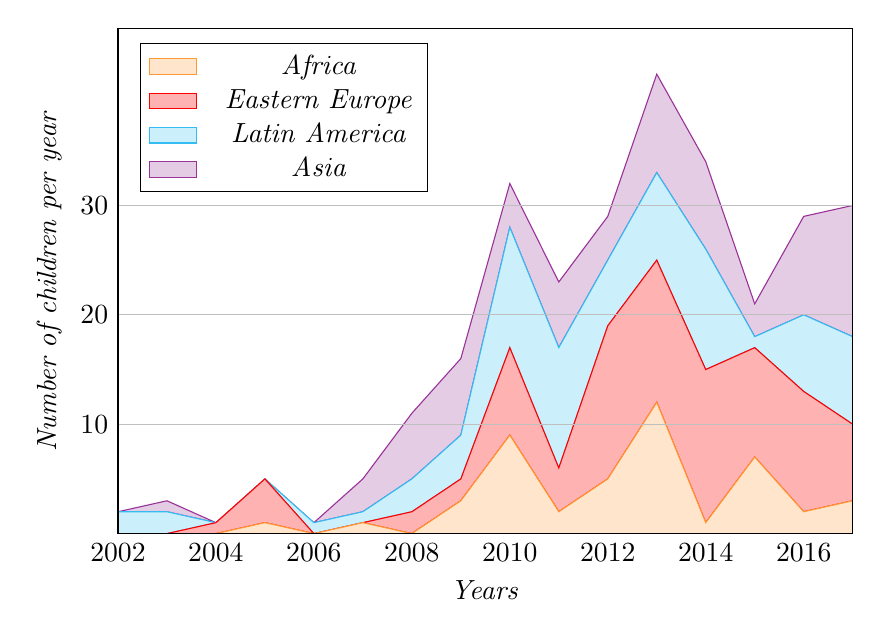
\begin{tikzpicture}
	\begin{axis}[
		stack plots=y,
		area style,
		enlarge x limits=false,
		enlarge y limits=upper,
		width=0.9\textwidth,
		height=8cm,
		xlabel = \textit{Years},
         ylabel = \textit{Number of children per year},
         ytick = {10, 20, 30},
         ytick style={draw=none},
         xtick style={draw=none},
         x tick label style={/pgf/number format/.cd,%
          scaled x ticks = false,
          set thousands separator={},
          fixed},
         y tick label style={/pgf/number format/.cd,%
          scaled y ticks = false,
          set thousands separator={},
          fixed},
         ymajorgrids=true,
         legend style={column sep=8pt},
         legend pos = north west]
    \addplot [draw={orange!80!white},fill={orange!20!white}] coordinates %Africa
		{(2002, 0) (2003, 0) (2004, 0) (2005, 1) (2006, 0) (2007,1 ) (2008, 0) (2009, 3) (2010, 9) (2011, 2) (2012, 5) (2013, 12) (2014, 1) (2015, 7) (2016, 2) (2017, 3)} 
		\closedcycle;
		\label{figdata:africa}
	\addplot coordinates % Eastern Europe
		{(2002, 0) (2003, 0) (2004, 1) (2005, 4) (2006, 0) (2007, 0) (2008, 2) (2009, 2) (2010, 8) (2011, 4) (2012, 14) (2013, 13) (2014, 14) (2015, 10) (2016, 11) (2017, 7)} 
		\closedcycle;
		\label{figdata:easterneurope}
	\addplot [draw={cyan!80!white},fill={cyan!20!white}] coordinates % Latin America
		{(2002, 2) (2003, 2) (2004, 0) (2005, 0) (2006, 1) (2007, 1) (2008, 3) (2009, 4) (2010, 11) (2011, 11) (2012, 6) (2013, 8) (2014, 11) (2015, 1) (2016, 7) (2017, 8)} 
		\closedcycle;
		\label{figdata:latinamerica}
		\addplot [draw={violet!80!white},fill={violet!20!white}] coordinates  % Asia
		{(2002, 0) (2003, 1) (2004, 0) (2005, 0) (2006, 0) (2007, 3) (2008, 6) (2009, 7) (2010, 4) (2011, 6) (2012, 4) (2013, 9) (2014, 8) (2015, 3) (2016, 9) (2017, 12)} 
		\closedcycle;
		\label{figdata:asia}
		\legend{\textit{Africa},\textit{Eastern Europe},\textit{Latin America},\textit{Asia}}
	\end{axis}
\end{tikzpicture}
\caption{Our population distribution - Total of children visited via the screening protocol, stratified by geographic area of origin}
\label{fig:populationperyear}
\end{figure}

\subsection{Inclusion and exclusion criteria}\label{sub:inclusionandexclusioncriteria}
All internationally adopted children brought to the \textit{San Vito al Tagliamento} GLNBI Center for medical attention, who underwent the GLNBI diagnostic and aiding protocol in the considered period of time, were included in the study. Only three children were excluded, due to the lack of information, because of voluntary early withdraw from the screening protocol.

The choice for so broadly defined inclusion criteria was made on the precise intent of the study: describing, as truthfully as possible, the health status of international adoptees. Therefore, the study group had to be as similar as possible as the population under exam. Moreover, this was meant to be a descriptive study, so the risk for confounders was considered limited, allowing us to consider the close-to-be entirety of the examined children.

As expressed in Section \ref{sec:thepopulationinexam}, we consider our study group to be highly representative of the population in exam (international adoptees).

\section{The dataset}\label{sec:dataset}
For the dataset, Microsoft Excel (Version 16.17) was chosen as the database environment, because of its widespread use and its gentle learning curve. The program ran on an early 2015 MacBook Pro with the operating system MacOS High Sierra (version 10.13.6).

The data was collected on an Excel spreadsheet during the years, normally twice per years, during the whole study period. The doctors working at San Vito al Tagliamento GLNBI Center meticulously inserted the children's information in the dataset.

In the Introduction to Appendix \ref{chap:appendixvbaexpressions}, on page \pageref{chap:appendixvbaexpressions}, Table \ref{tab:columnparameter} portrays the spreadsheet's full column-parameter correspondence, including units of measurement or cell type and a short description.

\section{Dataset elaboration}\label{sec:datasetelaboration}
At this point, it should be clear how data were collected, from which population of patients, and how this data was stored. In the following sections, it will be explained how the data was handled in order to produce the results illustrated in Chapter \ref{chap:results} on page \pageref{chap:results}. In particular, specific expressions were set up in the Excel spreadsheet via the VBA programming language, in order to understand which registered values were pathological and which were not (see Section \ref{sub:vbaexpressions}). In Section \ref{sub:cutoffvalues} it will be explained how and which cut-off values were chosen for this study and later implemented in the dataset elaboration and lastly, in Section \ref{sub:parasites}, a particular mention will be made on gastrointestinal parasites.

\subsection{VBA expressions}\label{sub:vbaexpressions}
In order to allow a precise statistical analysis, the dataset had to be tuned for this purpose. This was achieved via the implementation of VBA expressions in the Excel spreadsheet in \textit{ad hoc} columns. In particular, they were used to understand whether a specific value was pathological or not. This method was applied to:

\begin{itemize}
	\item Age in years (in Section \ref{asec:ageinyears})
	\item The geographic area of origin (in Section \ref{asec:geographicarea})
	\item Weight and height (in Section \ref{asub:patweightandheight})
	\item Haemoglobin (in Section \ref{asub:pathaemoglobin})
	\item MCV (in Section \ref{asub:patmcv})
	\item Circulating iron (in Section \ref{asub:patiron})
	\item Ferritin (in Section \ref{asub:patferritin})
	\item Vitamin D (in Section \ref{asub:patvitaminD})
	\item Parasitic infections and their groupings (in Sections \ref{asec:parasiticinfections}, \ref{asub:parasitespos}, and \ref{asub:parasitegrouping})
\end{itemize}

An explained overview of all the employed expressions can be found in Appendix \ref{chap:appendixvbaexpressions} on page \pageref{chap:appendixvbaexpressions}.

\subsection{Cut-off values}\label{sub:cutoffvalues}
At this point, it was necessary to understand which values of each parameter were to be considered positive, negative or anything in between. Therefore, cut-off values were established via an extensive research of the most recent medical literature. Every parameter will be now discussed on its own in the following sections.

\subsubsection{Height and Weight}\label{sub:heightandweight}
According to \cite{height1}, \cite{height4}, and \cite{height5} height and weight are fundamental parameters to appropriately establish whether a child is generically ill, as many infancy diseases disturb statural and ponderal growth; they can alter the first, the latter or both axes. We decided to focus on height and weight mainly as markers of malnutrition or chronic systemic disease.

Despite medical literature being unanimously decisive on setting the cut-off for both height and weight at the \nth{3} percentile (see \cite{height1}, \cite{height2} (from WHO), and \cite{height3}), we decided to consider pathological values under the \nth{10} percentile instead. This finds reason in that we preferred losing on some specificity, but ensuring the best sensibility, rather than the opposite. Precisely measuring a child may be a hard task, and growth curves may not always be coherent with one another, so we preferred to stick to \textit{``better safe than sorry"}. 

\subsubsection{Haemoglobin}\label{sub:haemoglobin}
Any physician knows that determining whether an haemoglobin value is pathological or not is impossible without any other knowledge of the patient's demographic information, physiological state, usual habits, \textit{etc}\dots The major factors that modulate haemoglobin serum levels are the following:
\begin{enumerate}
	\item Age: main one when studying a pediatric population.
	\item Sex: not relevant in pediatric age.
	\item Altitude: wasn't considered in our study, because of the impossibility of retrieving such an information from adoption records.
\end{enumerate}
Therefore, we elaborated the scheme illustrated in Table \ref{tab:cutoffhaemo}, based on the World's Health Organization (WHO) international 2017 guidelines. These can be found at \cite{Hbcutoff}. As briefly explained above, not having to consider sex or altitude made studying anemias much easier.

%Begin Table on Cutoff of Haemoglobin
\begin{table}[H]
   \centering
   \begin{tabular}{l c c c c}
   	  & & \multicolumn{3}{c}{Anemia\footnotemark[1]}\\
   	 \cline{3-5}
      Population & Non-anemia\footnotemark[1] & Mild\footnotemark[2] & Moderate & Severe\\
      \hline
      Children 6-59 months of age & $\geqslant 110$ & $100-109$ & $70-99$ & $\leqslant 69$\\
      Children 5-11 years of age & $\geqslant115$ & $110-114$ & $80-109$ & $\leqslant 79$\\
      Children 12-14 years of age & $\geqslant120$ & $110-119$ & $80-109$ & $\leqslant 79$\\
      Non-pregnant women & $\geqslant120$ & $110-119$ & $80-109$ & $\leqslant 79$\\
      Pregnant women & $\geqslant110$ & $100-109$ & $70-99$ & $\leqslant 69$\\
      Men & $\geqslant130$ & $110-129$ & $80-109$ & $\leqslant 79$\\
   \end{tabular}
   \caption{Employed haemoglobin cut-off values.}
    \source{World's Health Organization international 2017 guidlines for the diagnosis and treament of anemia (see \cite{Hbcutoff})}
    \label{tab:cutoffhaemo}
\end{table}

Therefore, based on haemoglobin serum levels, children were stratified in:
\begin{enumerate}
	\item Non-Anemia
	\item Anemia
	\begin{itemize}
		\item Mild
		\item Moderate\footnotemark[2]
		\item Severe
	\end{itemize}
\end{enumerate}

\footnotetext[1]{All haemoglobin values are expressed in $\si{\gram/\litre}$}
\footnotetext[2]{\textit{Mild} is a misnomer: iron deficiency is already advanced by the time anemia is detected. The deficiency has consequences even when no anemia is clinically apparent.}

A full technical overview of how this was implemented in the dataset elaboration can be found at Section \ref{asub:pathaemoglobin} on page \pageref{asub:pathaemoglobin}.

\subsubsection{MCV}\label{sub:mcv}
The Mean Corpuscular Value (MCV) was used in order to identify primarily genetic diseases ($\beta$-thalassemia minor) and carential states (iron, vitamin $B_{6}$ and $B_{12}$ deficiencies). In particular, it allowed us to separate macrocytic and microcytic anemias. The mean physiological value for MCV depends on numerous factors:

\begin{enumerate}
	\item Sex
	\item Age
	\item Alcohol and nutritional intakes
	\item Hematopoietic functionality and normal distribution of haemoglobin variants
	\item Endocrinological disorders (\textit{a.e.} hypothyroidism)
	\item Chronic intoxication (\textit{a.e.} lead poisoning)
	\item Consumption of many different medications (\textit{a.e. colchicine, heparin, estrogens, phenytoin, nitrofurantoin, triamterene,} and \textit{trimethoprim})
\end{enumerate}

Therefore we based our cut-off values on a recent review published on the International Journal of Laboratory Hematology (see \cite{MCVferritincutoff}), which evaluated these parameters in a pediatric population. Table \ref{tab:cutoffmcv} summarizes how these values were distributed; moreover, the table shows also ferritin cut-off, because the same review was employed in that parameter as well.

%Begin Table on Cutoff of Haemoglobin
\begin{table}[H]
   \centering
   \begin{tabular}{l r r c r r}
   	  & \multicolumn{2}{c}{Female} & & \multicolumn{2}{c}{Male}\\
   	 \cline{2-3} \cline{5-6}
      Age & Ferritin\footnotemark[4] & MCV\footnotemark[4] & & Ferritin\footnotemark[3] & MCV\footnotemark[4]\\
      \hline
      0-4 years of age & $8–82$ & $69–85$ & & $9–85$ & $71–85$\\
      5–9 years of age & $11–99$ & $75–89$ & & $12–94$ & $76–88$\\
      10–14 years of age & $8–94$ & $78–92$ & & $14–84$ & $76–90$\\
      15-19 years of age & $6–109$ & $77–94$ & & $20–191$ & $78–93$\\
      20-24 years of age & $7–129$ & $78–95$ & & $35–318$ & $82–94$\\
   \end{tabular}
   \caption{Employed MCV cut-off values.}
    \source{Åsberg et al. on International Journal of Laboratory Hematology (see \cite{MCVferritincutoff})}
    \label{tab:cutoffmcv}
\end{table}

\footnotetext[3]{All ferritin values are expressed in $\si{\nano\gram/\milli\litre}$}
\footnotetext[4]{All MCV values are expressed in $\si{\femto\litre}$}

A full technical overview of how this was implemented in the dataset elaboration can be found at Section \ref{asub:patmcv} on page \pageref{asub:patmcv}.

\subsubsection{Ferritin}\label{sub:ferritin}
Serum ferritin dosage is a direct marker of the patient's iron storage status. Thus, we recorded its value to further understand the etiologic nature of anemias in our population. The employed cut-off values can be found in Table \ref{tab:cutoffmcv} and are expressed in $\si{\nano\gram/\milli\litre}$.

A full technical overview of how this was implemented in the dataset elaboration can be found at Section \ref{asub:patferritin} on page \pageref{asub:patferritin}.

\subsubsection{Circulating Iron}\label{sub:iron}
The serum circulating iron value was defined as normal if it was included in the interval $16–129 \si{\micro\gram/\deci\litre}$, extremes included. This parameter was considered just as a countercheck for establishing the patient's iron storage status, that we deduced from serum ferritin.

A full technical overview of how this was implemented in the dataset elaboration can be found at Section \ref{asub:patiron} on page \pageref{asub:patiron}.

\subsubsection{Vitamin D}\label{sub:vitaminD}
Vitamin D deficiency and insufficiency are a major health issue in internationally adopted children, as explained in \ref{sec:roleofpediatrician} on page \pageref{sec:roleofpediatrician}, because of the profound change in latitude they experience during the adoption phase, or because of malnutrition combined with lack of solar exposure during pre-adoptive care, usually in orphanages. Thus, we dosed serum levels of calcifediol, also known as calcidiol, 25-hydroxycholecalciferol, or 25-hydroxyvitamin D (abbreviated $25(OH)D$).\\
Recent literature has recently openly discussed how vitamin D deficiency should be defined, especially in pediatric age, and therefore how what we should consider a healthy intake. The general international consensus states that to define Vitamin D serum cut-off values (intended as 25-hydroxyvitamin D), alkaline phosphatase and calcium serum levels should be taken into acquaintance so to determine a healthy bone development, ignoring the now well-known vitamin D extra-skeletal effects. The strongest recommendation for this comes from the letter addressed to BMJ from the British Society of Pediatric Radiology and child protection and nutrition committees of the Royal College of Pediatrics and Child Health in \cite{vitDcutoff_letter}. Moreover, \cite{vitDcutoff1}, a statistically strong and recent Italian review on a pediatric population, supports this statement, just as the reviews in \cite{vitDcutoff2} and \cite{vitDcutoff3}.

Table \ref{tab:cutoffvitD} summarizes the cut-off values, resulting from this approach. Since vitamin D serum levels are variably expressed both in $\si{\nano\gram/\milli\litre}$ and $\si{\nano\mol/\litre}$, both have been included in the following table. For this study, $\si{\nano\gram/\milli\litre}$ were used because this unit of measurement was the one used by our laboratories.

%Begin Table on Cutoff of Haemoglobin
\begin{table}[H]
   \centering
   \begin{tabular}{l c r r r r}
      Unit of Measurement & Sufficiency & Insufficiency & Deficiency & Severe Deficiency\\
      \hline
      $\si{\nano\gram/\milli\litre}$ & $\geqslant 20$ & $19–10$ & $9–4$ & $\leqslant 3$\\
      $\si{\nano\mol/\litre}$ & $\geqslant 50$ & $49–25$ & $24–10$ & $\leqslant 9$\\
   \end{tabular}
   \caption{Employed Vitamin D cut-off values.}
    \source{Saggese G et al. in ``Vitamin D in pediatric age: consensus of the Italian Pediatric Society and the Italian Society of Preventive and Social Pediatrics, jointly with the Italian Federation of Pediatricians" (see \cite{vitDcutoff1})}
    \label{tab:cutoffvitD}
\end{table}

Based on our laboratory findings we, therefore, scored the child's vitamin D status from 0 to 3, dividing their serum levels in:

\begin{itemize}
	\item Sufficient
	\item Insufficient
	\item Deficient
	\item Severely Deficient
\end{itemize}

A full technical overview of how this was implemented in the dataset elaboration can be found at Section \ref{asub:patvitaminD} on page \pageref{asub:patvitaminD}.

\subsection{Parasites grouping}\label{sub:parasites}
Gastrointestinal infestations are a common disease in internationally adopted children, as stated in \ref{sec:roleofpediatrician}. We found 8 different \textit{genera}, most of them co-infecting the same child. Because of the scarceness of data per genus, though, we decided to group them up into two separate groups, to increase statistical significance.

The found pathogens are the following:

%Custom list of Parasites in grouping
\begin{enumerate}[leftmargin=6em]
	\item [\textbf{Group 1}:] Parasites usually responsible for gastrointestinal bleeding and, therefore, iron-deficient low-ferritin microcytic anemia. These included:
		\begin{enumerate}[label=\alph*)]
			\item Entamoeba
			\item Ancylostoma
			\item Trichuris
		\end{enumerate}
	\item [\textbf{Group 2}:] Parasites usually responsible for gastrointestinal malabsorption. These included:
		\begin{enumerate}[label=\alph*)]
			\item Giardia
			\item Strongyloides
			\item Hymenolepis
			\item Blastocystis
			\item Endolimax
		\end{enumerate}
\end{enumerate}

A full technical overview of how this was implemented in the dataset elaboration can be found at Section \ref{asec:parasiticinfections} on page \pageref{asec:parasiticinfections}.

%QUI SI PARLA DI PERCHE LI HAI DIVISI IN DUE GRUPPI E COME (SUL FATTO CHE FOSSERO ANEMIZZANTI O MENO) E POI VEDIAMO I RISULTATI
% IN \cite{GNLBIexp} C'è una tabella con cui comparare i risultati!!
%Fai riferimento all'Appendice corrispondente.

\section{Statistical Analyses}\label{sec:statisticalanalyses}
The population-describing analyses were conducted using relative frequencies and percentages for categorical variables, and means and standard deviations or medians and inter-quartile intervals for continuous ones. We preferred to use the latter because the scarcity of data prevented us from checking for normal distribution.\\
Nonparametric tests, such as the \textit{Mann-Whitney-Wilcoxon rank-sum test} or \textit{Kruskal-Wallis equality-of-populations rank test}, were employed to evaluate the difference between continuous variables in different groups. One test or the other was performed based on the number of groups, case by case: if two, the \textit{Mann-Whitney-Wilcoxon} test was used, if more than two, \textit{Kruskal-Wallis} test, instead. To study the relation between two dichotomous variables, or one dichotomous and one categorical, we used the \textit{two-tailed Fisher's exact test} and, to study whether a dichotomous event was associated with one or more independent variables, we preferred using logistic regression.\\
Lastly, in order to study the correlation between continuous variables, we preferred using \textit{Spearman's rank correlation}.

All statistical analyses were conducted using the Stata/IC software, version 14.2 (StataCorp LLC, College Station, USA).